% !TEX root = ../main.tex
\documentclass[../main.tex]{subfiles}

\begin{document}
\section{Asset management}

\subsection{Upload process and storage}

Asset upload is done though the \texttt{ipxe/upload} endpoint. The endpoint accepts a POST request with the \texttt{multipart/form-data} content type.
Multiple files can be uploaded at once. An array of asset URLs is returned in the response body.

The file upload and file store is handled by \texttt{multer} \cite{multer}, a middleware for Express.
The middleware stores uploaded files in the fielesystem in the location specified by the configuration file.

\begin{listing}[H]
  \tsfile{implementation/code/cli/multer-config.ts}
  \caption{Multer configuration}
\end{listing}

By defualt, multer does not remove files if the upload process fails. This is not desirable, as it would lead to a buildup of unused files.
To fix this behavior an event handler is added to the request \textbf{abort} event which removes the uploaded files from the filesystem.

Uploaded files are stores in flat struture in the filesystem. To avoid name collistions a unique identifier is generated for each file.

\begin{figure}[H]
  \centering
  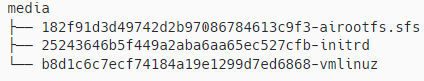
\includegraphics{file-tree/media-tree.png}
  \caption{Contents of the directory where uploaded files are stored}
\end{figure}

For each file uploaded file a record is created in the database which stores the file's metadata such as the original file name and the path where the file is stored.

\begin{figure}[H]
  \centering
  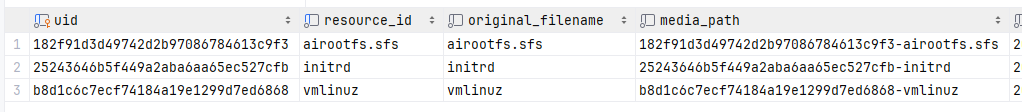
\includegraphics[width=\textwidth]{assets/file-entries-database.png}
  \caption{File metadata entries in the database}
\end{figure}

\subsection{Web interface}

The web interfaces shows a list of assets stored in the system using a \texttt{DataTable} component which makes it easy to sort filter and manage the data.
Additionally, a dropzone component is used to allow users to upload files by dragging and dropping them on the page.

\begin{figure}[H]
  \centering
  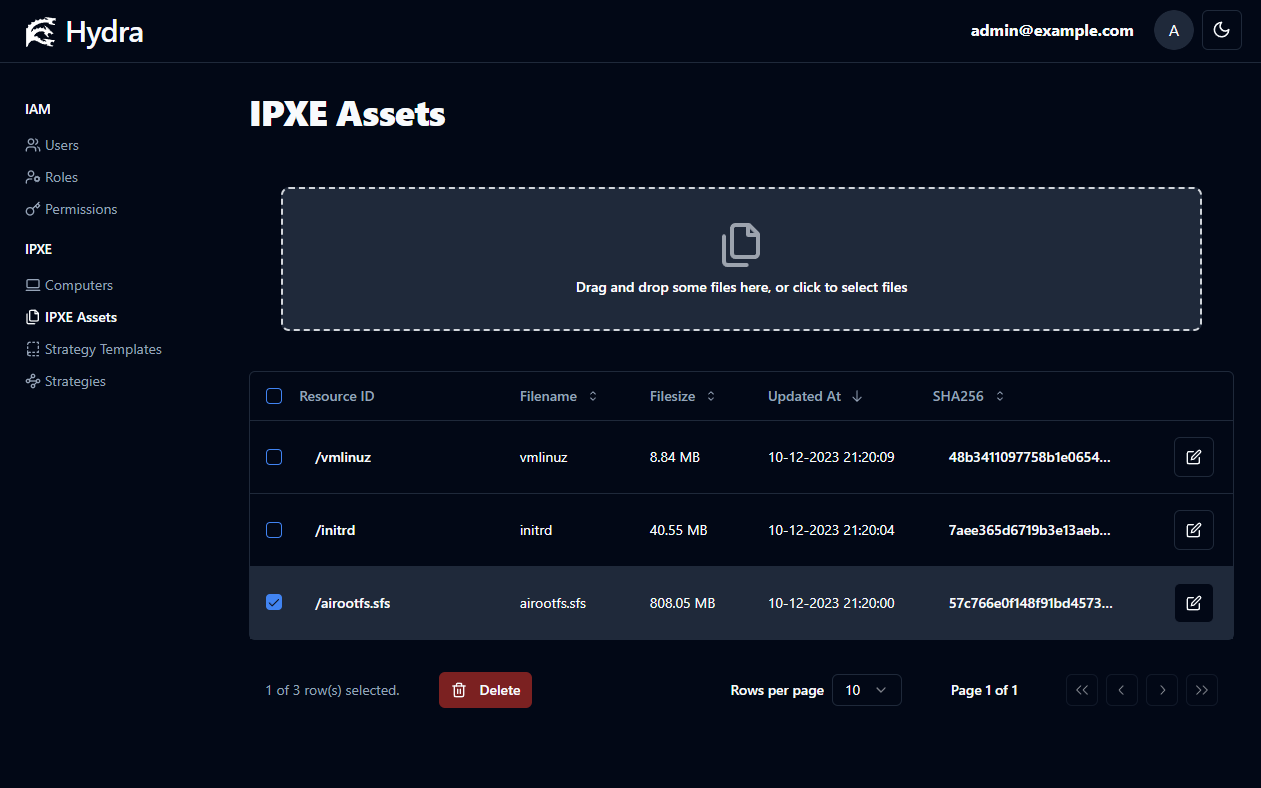
\includegraphics[width=\textwidth]{assets/web_ui.png}
  \caption{Assets web interface}
\end{figure}

When a file is uploaded, the web interface shows a progress bar which indicates the progress of the upload.

\begin{figure}[H]
  \centering
  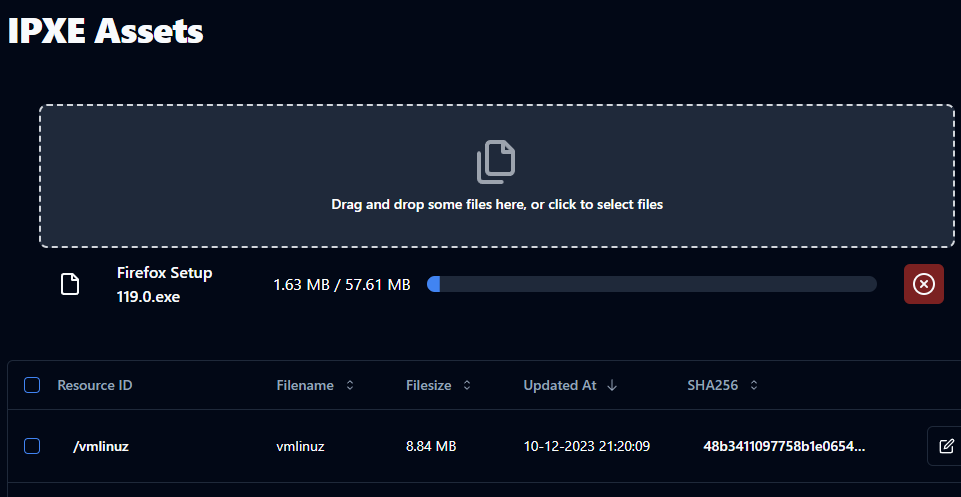
\includegraphics[width=\textwidth]{assets/upload_progress.png}
  \caption{Upload progress when uploading asset}
\end{figure}

After the upload is complete a random resource identifier is generated for the asset which is used to access the asset.
This identifier is hown in the table in \texttt{Resource ID} column.
For example if the resource identifier is \texttt{a1b2c3d4} the asset can be accessed at \texttt{http://server-host/api/ipxe/assets/a1b2c3d4}.
It is possible to change the resource indentifier by clicking on the \texttt{Edit} button in the \texttt{Actions} column.
Resource identifiers can have multiple segments, for example \texttt{a1b2c3d4/e5f6g7h8}, in which case the asset can be accessed at \texttt{/api/ipxe/assets/a1b2c3d4/e5f6g7h8}.

\begin{figure}[H]
  \centering
  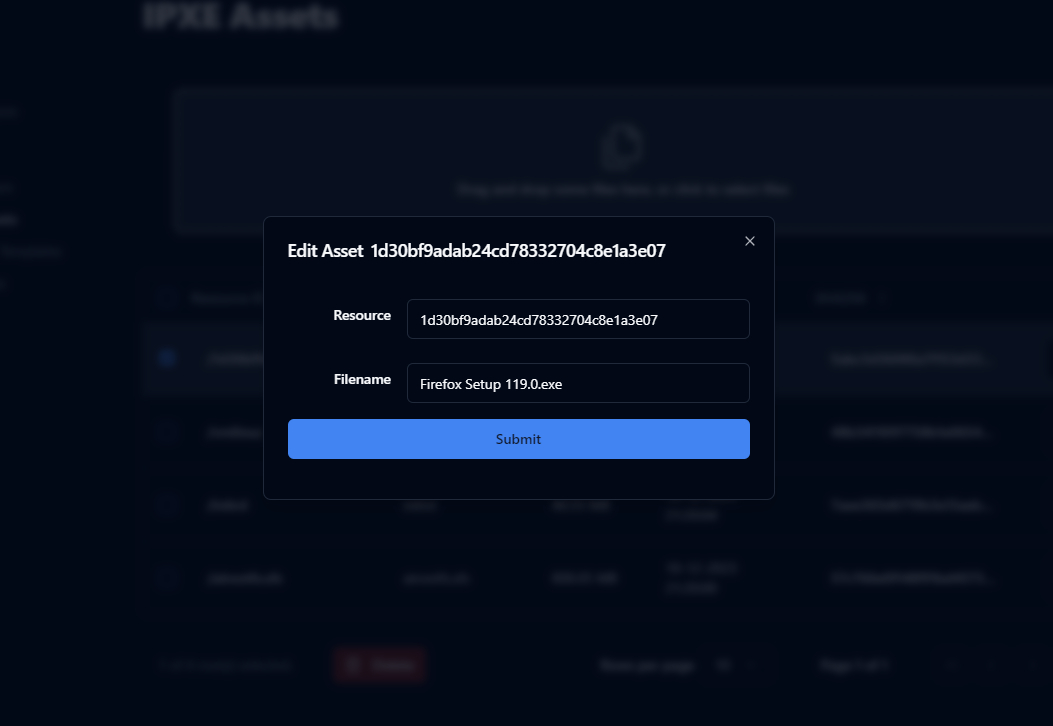
\includegraphics[width=\textwidth]{assets/editing_asset.png}
  \caption{Editing resource identifier}
\end{figure}

For the SystemRescue booting process the following set of assests is used as shown in figure \ref{fig:sysrescue-assets}.

\begin{figure}[H]
  \centering
  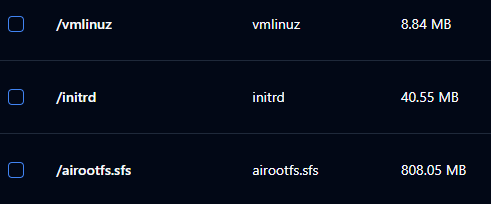
\includegraphics{assets/sysrescue_assets.png}
  \caption{SystemRescue assets}
  \label{fig:sysrescue-assets}
\end{figure}

\end{document}